\chapter{Graph Grammars}\label{ch:gts}

The theory of graph grammars and graph transformation systems is based on the application of rules that are able to modify graphs. Using this framework, it is possible to model complex systems as graph transformation systems, where graphs represent the system states and the rules model transitions between states.

Graph grammars have a wide application in computer science, not only because graphs are very natural and intuitive way to model complex situations, but also because it is possible to reason about several properties of the modelled systems using its formalism~\cite{Ehrig2006,Rozenberg1997}.

We now review the basic concepts and analysis techniques for graph transformations that are used in this work. We use the algebraic approach, which is based on category theory. The reader is assumed to be familiar with categorial concepts, but a brief review of the main concepts used in this thesis is presented in appendix~\ref{app:category-theory}.

\begin{definition}[Graph] A graph is a tuple $G = \left(V,E,s,t\right)$ where: $V$ is a set of nodes, $E$ is a set of Edges and $s,t : E \rightarrow V$ are two total functions that map each edge in $E$ to its source and target in $V$.

\end{definition}

\begin{example}[Graph]\label{def:graph} Figure~\ref{fig:gts:graph} shows a simple graph $G$ with $V = \{1,2,3,4\}$, $E = \{1,2\}$, $s =\{(1,1),(2,3)\}$ and $t = \{(1,2),(2,3)\}$.
\begin{figure}[!ht]
  \centering
  
\includegraphics[scale=0.6]{images/gts/graph}
  \caption{A graph example}\label{fig:gts:graph}
\end{figure}
\end{example}

\begin{definition}[Graph Morphism]\label{def:graph-morphism} Given two graphs $G_1,G_2$ with \mbox{$G_i = \left(V_i, E_i, s_i, t_i\right)$} for $i$ in $[1,2]$, a graph morphism $f : G_1 \rightarrow G_2$ between them is a pair $f = \left(f_V,f_E\right)$ where $f_V : V_1 \rightarrow V_2$ and $f_E : E_1 \rightarrow E_2$ are total functions that preserve the source and target functions, i.e. $f_V \circ s_1 = s_2 \circ f_E$ and $f_V \circ t_1 = t_2 \circ f_E$.
\end{definition}

\begin{example}[Graph Morphisms]Figure~\ref{fig:gts:compact-graph-morphism} shows three morphisms $f : G_0 \rightarrow G_1$, $g : G_0 \rightarrow G_2$ and $h : G_0 \rightarrow G_3$, which are a monomorphism, an epimorphism and a isomorphism, respectively.

  Morphism $f$ maps node $\Circle_1$ to $\Circle_a$, node $\Circle_2$ to $\Circle_b$ and edge $\curvearrowleft_1$ to $\curvearrowleft_q$; $g$ maps both nodes $\Circle_1$ and $\Circle_2$ to $\Circle_c$ and edge $\curvearrowleft_1$ to $\curvearrowleft_r$; and $h$ maps node $\Circle_1$ to $\Circle_d$, node $\Circle_2$ to $\Circle_e$ and edge $\curvearrowleft_1$ to $\curvearrowleft_s$.

  Figure~\ref{fig:gts:expanded-graph-morphism} shows the morphism $f$ in an expanded (explicit) notation. Both notations will be used through this work.
\begin{figure}[!ht]
  \centering
  \fbox{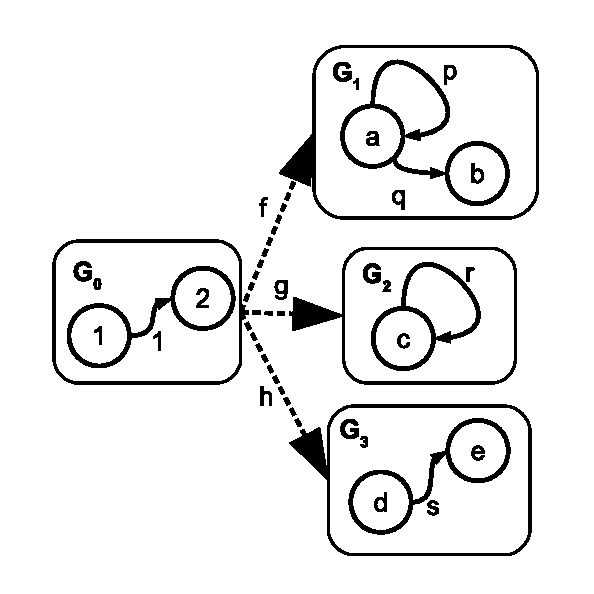
\includegraphics[scale=0.6]{images/gts/compact-graph-morphism}}
  \caption{Graph morphisms example}\label{fig:gts:compact-graph-morphism}
\end{figure}

\begin{figure}[!ht]
  \centering
  \fbox{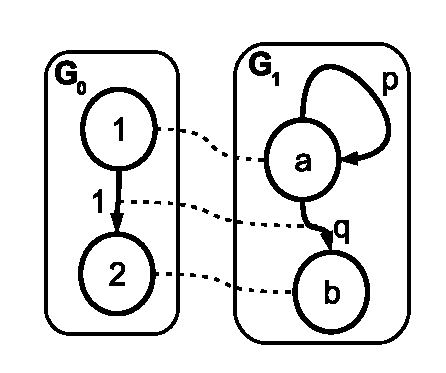
\includegraphics[scale=0.6]{images/gts/expanded-graph-morphism}}
  \caption{Expanded graph morphism example}\label{fig:gts:expanded-graph-morphism}
\end{figure}
\end{example}

\begin{definition}[Typed Graph and Typed Graph Morphism] A type graph is a distinguished graph $TG = \left(V_{TG},E_{TG},s_{TG},t_{TG}\right)$ where $V_{TG}$ and $E_{TG}$ are called the node and edge type alphabets, respectively.

  A typed graph is a pair $G^T = \left(G, type\right)$ consisting of a graph $G$ and a graph morphism $type : G \rightarrow TG$.

  Given two typed graphs $G^T_1 = \left(G_1,type_1\right)$ and $G^T_2 =\left(G_2,type_2\right)$, a typed graph morphism $f : G^T_1 \rightarrow G^T_2$ is a graph morphism $f : G_1 \rightarrow G_2$ such that $type_2 \circ f = type_1$:

\diagram{
  G_1\ar[rr]^{f}\ar[dr]_{type_1} & & G_2\ar[dl]^{type_2}\\
  \ar@{}[rur]|{=}& TG &
}
\end{definition}

\begin{example}[Typed Graph and Typed Graph Morphism Example] Figure~\ref{fig:gts:typed-graphs} shows a type graph $T$, and four graphs $G_0, G_1, G_2, G_3$ where only $G_0$ and $G_1$ are valid \emph{T-typed} graphs. 
  
  Notice that $G_2$ can not be a \emph{T-typed} graph because type graph does not have a node of the type $\lozenge$, neither an edge type with source and target in the $\Square$ type. Similarly, $G_3$ is not a valid \emph{T-typed} graph because, although there is an edge type between a $\triangle$ and a $\Square$ types, the source must of this type of edge must be a $\Square$ and the target a $\triangle$.

  Figure~\ref{fig:gts:typed-graph-morphism} shows a typed graph morphism $f : G_0^T \rightarrow G_1^T$, where $f$ maps node $\Circle_a$ to $\Circle_1$, $\Square_b$ to $\Square_1$ and edge $\curvearrowleft_e$ to $\curvearrowleft_2$.
\begin{figure}[!ht]
  \centering
  \fbox{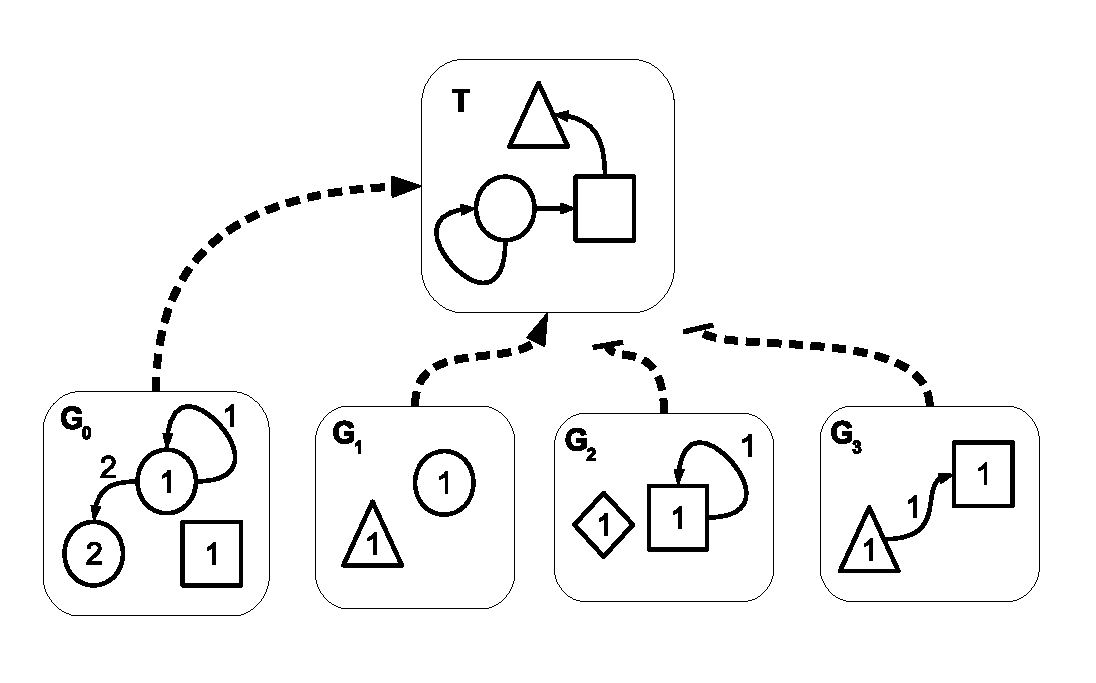
\includegraphics[scale=0.65]{images/gts/typed-graphs}}
  \caption{\emph{T-typed} valid and invalid graphs}\label{fig:gts:typed-graphs}
\end{figure}

\begin{figure}[!ht]
  \centering
  \fbox{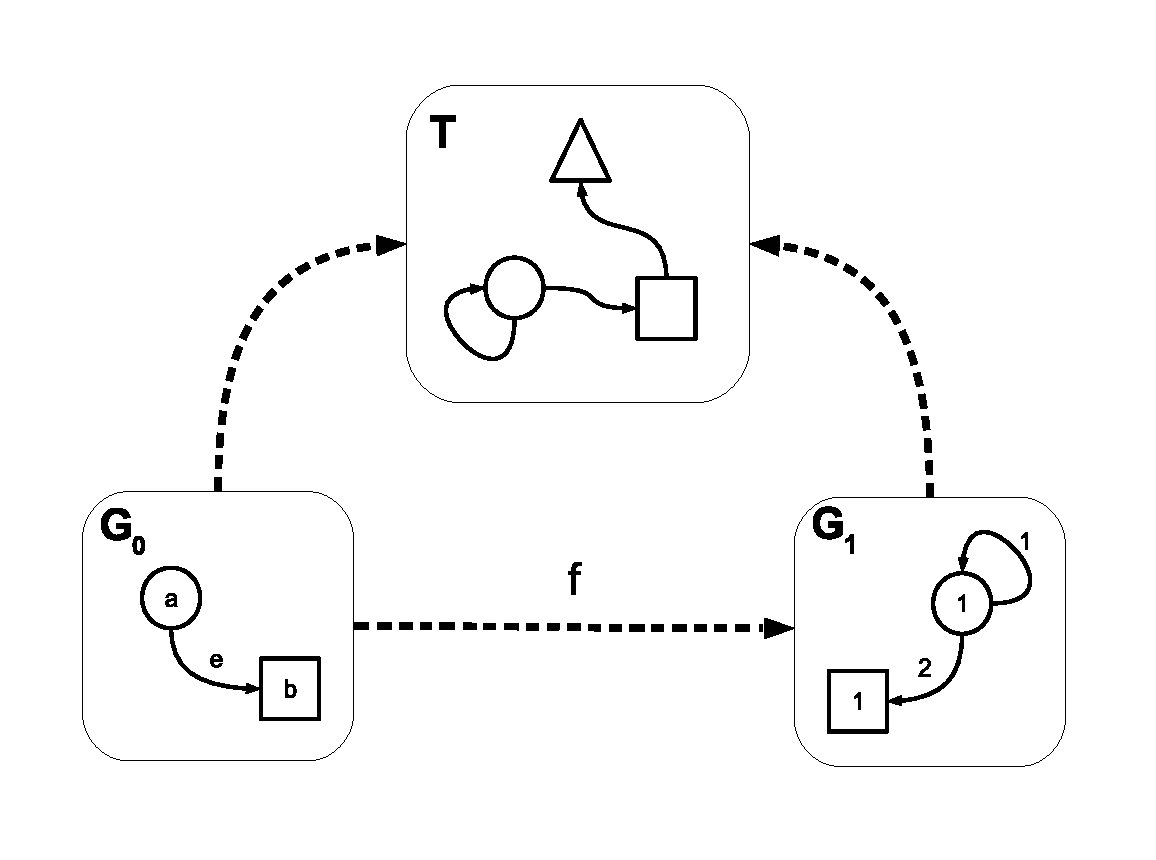
\includegraphics[scale=0.6]{images/gts/typed-graph-morphism}}
  \caption{A typed graph morphism}\label{fig:gts:typed-graph-morphism}
\end{figure}
\end{example}

\begin{remark}[Categories of Graphs and Typed Graphs] We call \cat{Graph} the category whose objects are graphs and arrows are graph morphisms. Similarly, we have that \cat{TGraph_T} is the category whose objects are $T-$typed graphs and whose arrows are $T-$typed graph morphisms.
\end{remark}

\iffalse
\begin{definition}[Positive Atomic Constraint] A \emph{positive} atomic (typed) graph constraint is of the form $PC\left(a\right)$, where $a : P \rightarrow C$ is a (typed) graph morphism. A (typed) graph $G$ satisfies $PC\left(a\right)$ if for every injective (typed) graph morphism $p : P \rightarrow G$ there is at least one injective (typed) graph morphism $q : P \rightarrow C$ such that $p = q \circ a$.

  A positive (typed) graph constraint with $a : \emptyset \rightarrow C$ is also notated $PC\left(C\right)$. Given a (typed) graph $G$, it satisfies $PC\left(C\right)$ if there is an injective (typed) graph morphism $q : C \rightarrow  G$.
\diagram{
  P\ar[rr]^{a}\ar[dr]_{p} & & C\ar[dl]^{q}\\
  \ar@{}[rur]|{=}& G &
}

\end{definition}

\begin{definition}[Negative Atomic Constraint]
A \emph{negative} atomic (typed) graph constraint is of the form $NC\left(a\right)$, where $a : P \rightarrow C$ is a (typed) graph morphism. A (typed) graph $G$ satisfies $PC\left(a\right)$ if for every injective (typed) graph morphism $p : P \rightarrow G$ there is no injective (typed) graph morphism $q : P \rightarrow C$ such that $p = q \circ a$.

  A negative (typed) graph constraint with $a : \emptyset \rightarrow C$ is also notated $NC\left(C\right)$. Given a (typed) graph $G$, it satisfies $NC\left(C\right)$ if there is no injective (typed) graph morphism $q : C \rightarrow G$.

\diagram{
  P\ar[rr]^{a}\ar[dr]_{p} & & C\ar[dl]|{|}^{q}\\
  \ar@{}[rur]|{=}& G &
}

\end{definition}

\begin{remark} It was shown in ~\cite{Ehrig2006} that negative atomic constraints do not give more expressive power. However, we introduced this concept because it makes easier to reason about some of the purposes of this thesis in a negative rather than a positive manner.%\tinytodo{related to the graph constraint definition, maybe this is not necessary}
\end{remark}

\begin{definition}[Graph Constraint] A (typed) graph constraint is a \emph{boolean} formula over atomic (typed) graph constraints, in such way that $true$, $false$ and every atomic constraint are also graph constraints. Also, if $c$ and $c_i$, with $i \in I$ for some index set $I$, are graph constraints, then $\neg c$, $\land_{i \in I} c_i$ and $\lor_{i \in I} c_i$ are also graph constraints.

  A graph $G$ satisfies a graph constraint $c$ (written $G \models c$) iff one of the following situations occurs:
  \begin{itemize}
    \item $c = true$
    \item $c$ is an atomic constraint $a$ and $G \models a$
    \item $c = \neg c'$ and $G \not\models c'$
    \item $c = \land_{i \in I}c_i$ and $G \models c_i$ $\forall i \in I$ 
    \item $c = \lor_{i \in I}c_i$  and $\exists i \in I$ such that $G \models c_i$
  \end{itemize}
\end{definition}

\begin{example}[Constraints Example]
\end{example}
\fi

\begin{definition}[Graph Rule]\label{def:graph-rule} A (typed) graph rule\footnote{Also called graph transformation rule or graph production.} \graphrule{} is a span of (typed) graph monomorphisms \lefthand{} and \righthand{}  where the (typed) graphs $L$, $K$ and $R$ are called the left-hand side, gluing graph and right-hand side, respectively.

  Given a (typed) graph rule $p$, its inverse rule is defined by \inversegraphrule.
\end{definition}

\begin{example}[Graph Rule Example and Notation] Figure~\ref{fig:gts:rule} shows an example of a graph rule which reads a node of the type $\Circle$, deletes a node of the type $\triangle$ and then creates a node of the type $\Square$ with an edge between the $\Circle$ and the \Square. 
  
Figure~\ref{fig:gts:rule-standard} presents the rule in the standard DPO notation, while Figure~\ref{fig:gts:rule-compact} depicts the same rule in a compact notation, where the gluing graph is omitted. Sometimes we will use the compact notation to make the figures smaller. Notice that the compact notation does not cause any semantic loss as the gluing graph can be obtained as the ``intersection'' between the left and right graphs, and the morphisms $l$ and $r$ as the inclusions of $K$ in $L$ and $R$, respectively.

\begin{figure}[!ht]
  \centering
  \begin{subfigure}[t]{.5\textwidth}
    \centerline{\fbox{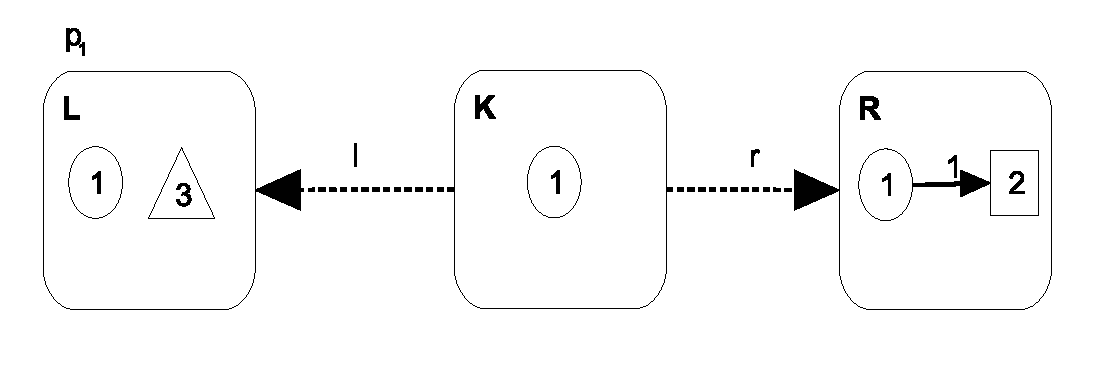
\includegraphics[scale=0.5]{images/gts/standard-dpo-rule}}}
    \caption{Standard DPO rule notation}\label{fig:gts:rule-standard}
  \end{subfigure}

  \begin{subfigure}[t]{.5\textwidth}
    \centerline{\fbox{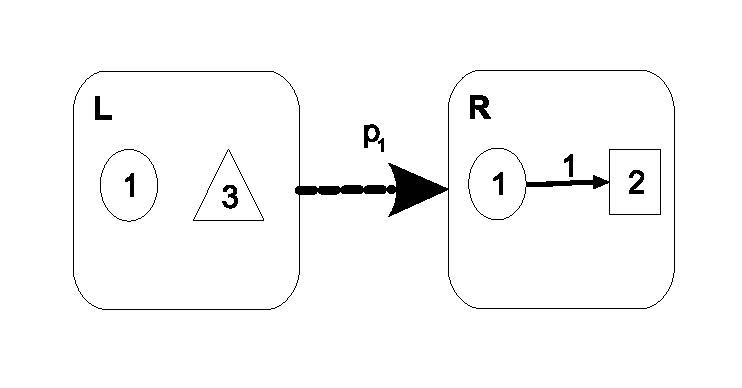
\includegraphics[scale=0.5]{images/gts/compact-dpo-rule}}}
    \caption{Compact DPO rule notation}\label{fig:gts:rule-compact}
  \end{subfigure}
  \caption{DPO graph rule}\label{fig:gts:rule}
\end{figure}
\end{example}

\begin{definition}[Graph Transformation] Given a (typed) graph rule \graphrule{} and a (typed) graph $G$ with a (typed) graph morphism \match, called match, a direct (typed) graph transformation $G \xRightarrow{p,m} H$ from $G$ to a (typed) graph $H$ is a double-pushout (DPO) diagram such as:

\diagram{
  L\ar[d]_{m}        & & K\ar[ll]_{l}\ar[rr]^{r}\ar[d]|{k} & & R\ar[d]^{m'}\\
  G\ar@{}[urr]|{\left(1\right)} & & D\ar[ll]^{f}\ar[rr]_{g}             & & H\ar@{}[ull]|{\left(2\right)}
}

  For \cat{TGraph_T} there are two conditions, called \emph{gluing conditions}, that must be satisfied so that the pushouts (1) and (2) exist and the rule graph rule can be applied:

\begin{itemize}
  \item the \emph{dangling condition} requires that no node can be deleted if it has incident edges that are not also deleted (otherwise the result of this deletion would not be a graph).  
  \item the \emph{identification condition} requires the match to not identify a deleted element with a preserved or (another) deleted one.
\end{itemize}

  \important{define what are ``deleted'' and ``preserved'' nodes}
\end{definition}

\begin{example}[Graph Transformation Examples] Figure~\ref{fig:gts:transformation-success} shows a transformation where the rule depicted in Figure~\ref{fig:gts:rule} is successfully applied over a graph instance $G_0$.

  Figure~\ref{fig:gts:transformation-fail} shows the same rule being applied over a graph instance $G_1$ which does not satisfy the gluing conditions, more specifically it does not satisfy the dangling condition.

\begin{figure}[!ht]
  \centering
  \begin{subfigure}[t]{.5\textwidth}
    \centerline{\fbox{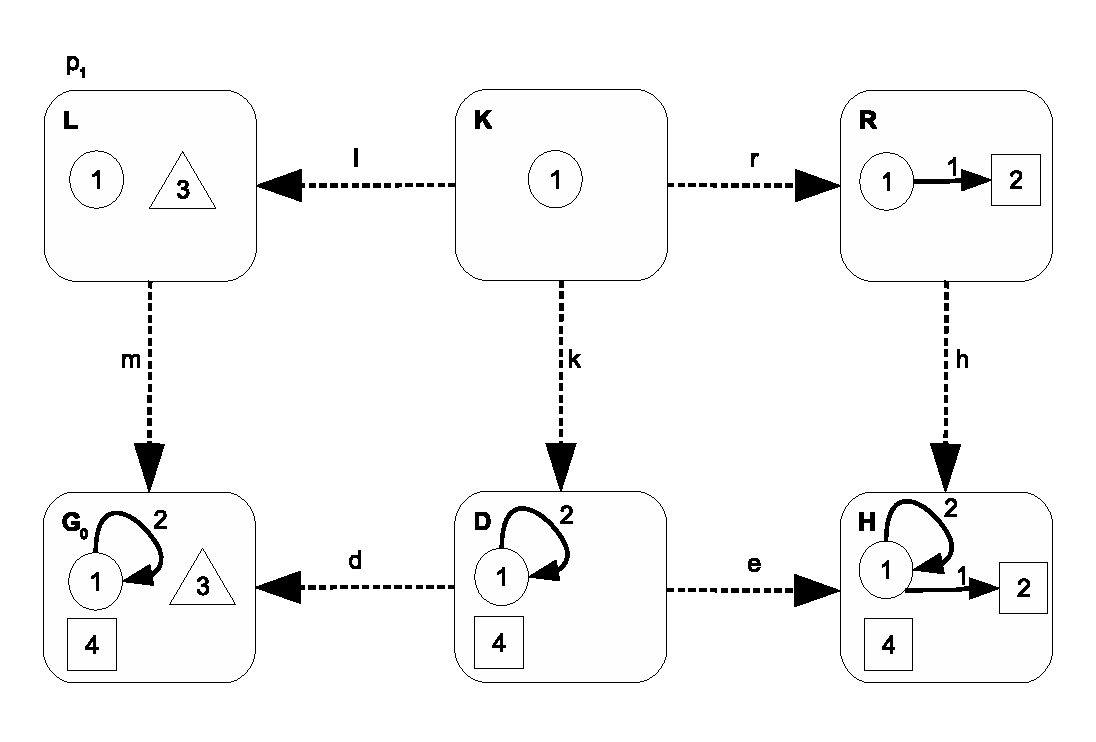
\includegraphics[scale=0.8]{images/gts/transformation}}}
    \caption{Successfully applied graph transformation}\label{fig:gts:transformation-success}
  \end{subfigure}

  \begin{subfigure}[t]{.5\textwidth}
    \centerline{\fbox{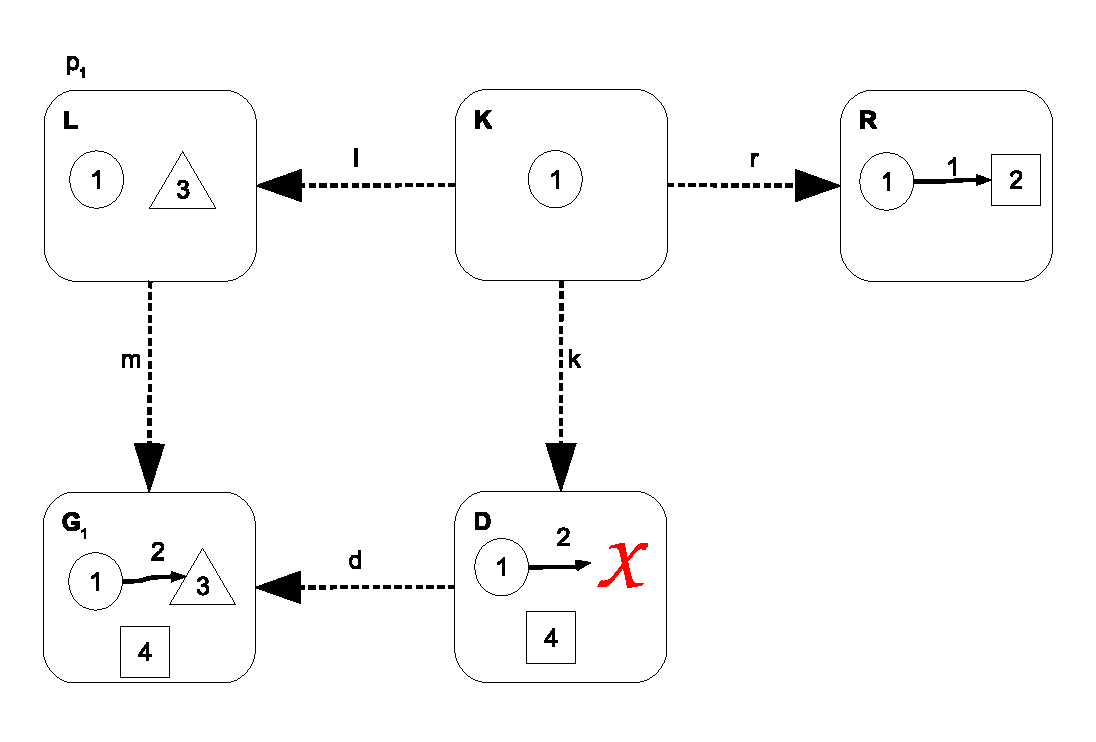
\includegraphics[scale=0.8]{images/gts/transformation-failed}}}
    \caption{Failing graph transformation due to the dangling condition}\label{fig:gts:transformation-fail}
  \end{subfigure}
  \caption{Graph transformation}\label{fig:gts:transformation}
\end{figure}
\end{example}

\important{put some text introducing nacs}

\begin{definition}[Negative Application Condition] A \emph{left} negative application condition over a graph rule \graphrule{} is of the form $NAC\left(n\right)$, where \nac{} is an arbitrary (typed) graph morphism. A match \match{} of a rule $p$ satisfies\footnote{When a NAC is satisfied it is also said that the NAC is \emph{not triggered} and vice versa.} $NAC\left(n\right)$ on $L$, written $m \models NAC\left(n\right)$, iff $\nexists$ $q : N \rightarrow G$ with $q$ injective and $q \circ n = m$.

\diagram{
  N\ar@{.>}[dr]|{|}_{q} & L\ar[d]^{m}\ar[l]_{n}\\
   & G
}

  A match \match{} satisfies a set \mbox{$NAC_L = \{NAC\left(n_i\right)|i \in I\}$} of left $NACs$, iff \mbox{$m \models NAC\left(n_i\right)$} $\forall i \in I$.

  Analogously, a \emph{right} negative application condition over a graph rule \graphrule{} is of the form $NAC\left(n\right)$, where \rightnac{} is an arbitrary (typed) graph morphism. A comatch \comatch{} of a rule $p$ satisfies $NAC\left(n\right)$ on $R$ (written \mbox{$m' \models NAC\left(n\right)$}) iff $\nexists$ $q : N \rightarrow H$ with $q$ injective and $q \circ n = m'$.

\diagram{
  R\ar[d]_{m'}\ar[r]^{n} & N\ar@{.>}[dl]|{|}^{q}\\
  H &
}
  Also, a comatch \comatch{} satisfies a set \mbox{$NAC_R = \{NAC\left(n_i\right)|i \in I\}$} of right $NACs$, iff $m' \models NAC\left(n_i\right)$ $\forall i \in I$.

\end{definition}

\begin{example}[NAC and NAC satisfiability] Figure~\ref{fig:gts:nacs:satisfied} shows a NAC that is satisfied (i.e. not triggered) over a match $m$, as there is no possible way of mapping the edge between $\Circle_1$ and $\Square_1$ in $N$ to an edge in $G_0$ such that the resulting triangle commutes. Therefore, if $G_0$ also satisfies the gluing conditions for the corresponding rule the transformation can be applied.

  On the other hand, Figure~\ref{fig:gts:nacs:triggered} shows a NAC that is triggered (i.e. not satisfied) over the match $m$: all the elements in $N$ can be mapped to $G_0$ such that the resulting triangle commutes. Therefore, even if $G_0$ satisfies the gluing conditions, the transformation can not be applied, as the pattern forbidden by the NAC was found on the instance graph.

\begin{figure}[!ht]
  \centering
  \begin{subfigure}[t]{.5\textwidth}
    \centerline{\fbox{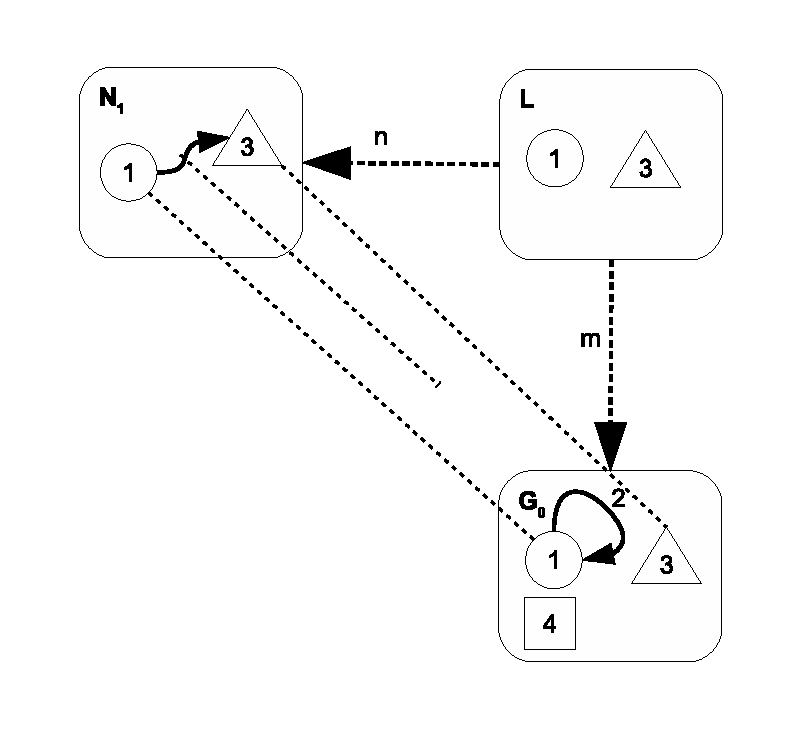
\includegraphics[scale=0.55]{images/gts/satisfied_nac}}}
    \caption{A satisfied NAC}\label{fig:gts:nacs:satisfied}
  \end{subfigure}%
  \begin{subfigure}[t]{.5\textwidth}
    \centerline{\fbox{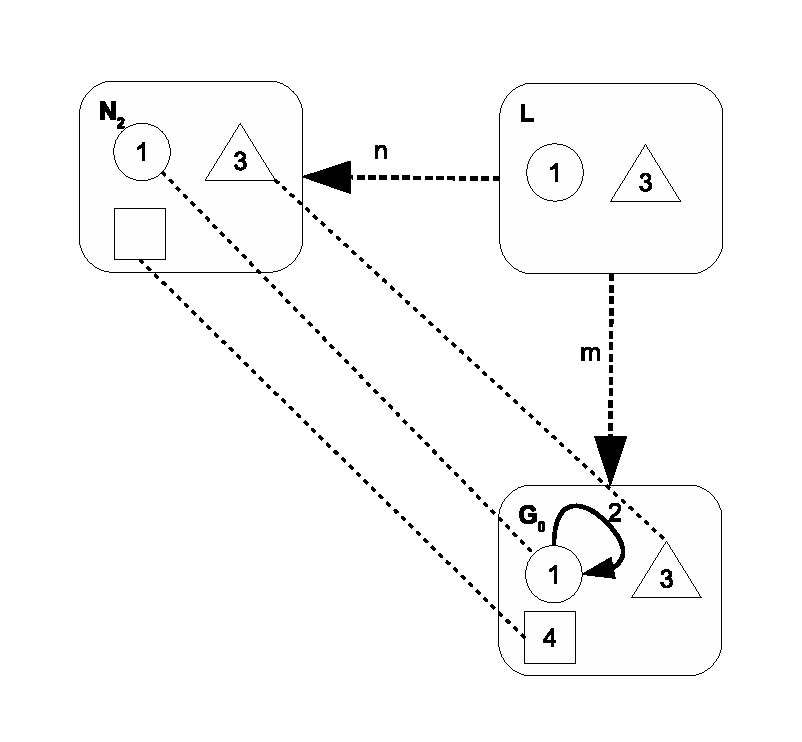
\includegraphics[scale=0.55]{images/gts/triggered_nac}}}
    \caption{A triggered NAC}\label{fig:gts:nacs:triggered}
  \end{subfigure}
  \begin{subfigure}[t]{.5\textwidth}
    \centerline{\fbox{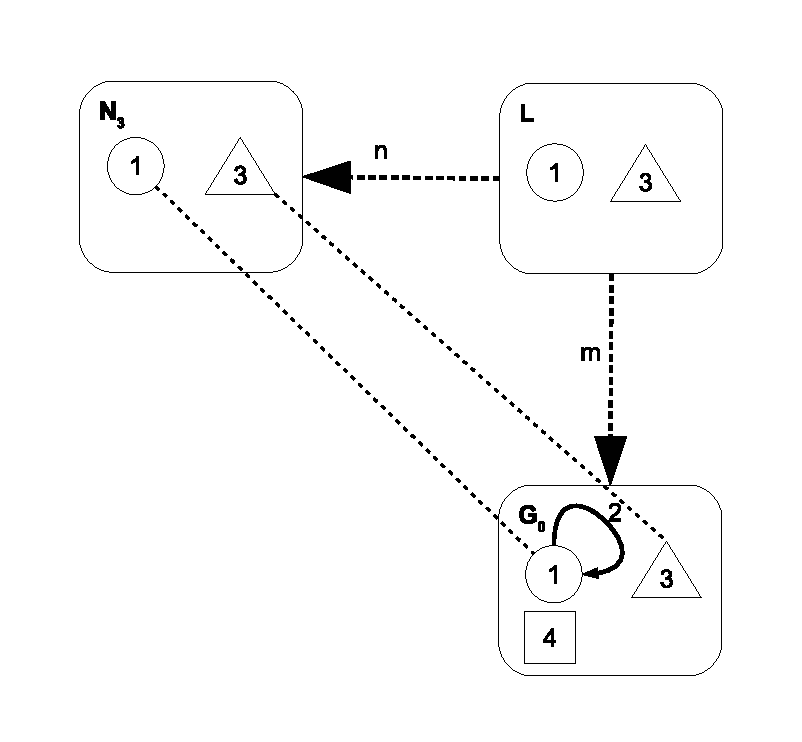
\includegraphics[scale=0.55]{images/gts/trivially_triggered_nac}}}
    \caption{A trivially-triggered NAC}\label{fig:gts:nacs:trivial}
  \end{subfigure}
  \caption{NACs and NAC satisfiability}\label{fig:gts:nacs}
\end{figure}
\end{example}

%\begin{assumption}[Left NACs] Unless stated otherwise, we will work with graph rules that have only left $NACs$ for the rest of this thesis. This is without loss of generality once right $NACs$ can be translated to left ones as it is shown in Definition~\ref{def:shift-nac}.
%\end{assumption}

\begin{definition}[Trivially-Triggered NACs] Given a $NAC(n)$, where $n : L \rightarrow \hat{L}$ is a isomorphism, and a match \match{} which is also a monomorphism, we call $NAC(n)$ a \emph{trivially-triggered NAC} as, for every monomorphic $m$, there will always exist a $q : \hat{L} \rightarrow G$ injective such that $q \circ n = m$.

  A trivially-triggered NAC $n : L \rightarrow \hat{L}$ is also notated $NAC(L)$. If a rule $p$ has a trivially-triggered NAC then $p$ can never be applied whatsoever, as the NAC will never be satisfied. An example of a trivially-triggered NAC is shown on Figure~\ref{fig:gts:nacs:trivial}.
\end{definition}

\begin{definition}[Graph Transformation System and Graph Grammar] A typed graph transformation system is a pair $GTS = \left(TG,P\right)$ where $TG$ is the type graph of the system and $P$ is a set of typed graph rules with NACs.

  A typed graph grammar is a pair $GG = \left(GTS,I\right)$ where $TGS$ is a typed graph transformation system and $I$ is a typed start graph. It can also be notated as $GG = \left(TG, I^{TG},P \right)$.

\end{definition}

\begin{example}[Mail Server Graph Transformation System] Fig~\ref{fig:gts:mail} depicts a graph transformation system that models a client-server scenario for a very simple e-mail application \important{(explain types)}. This system has only four actions: 

\begin{enumerate}
  \item \emph{sendMessage}: a client sends a message to a server,\tinytodo{fix arrow direction}
  \item \emph{getData}: a piece of data is obtained from a server,
  \item \emph{receiveMessage}: a server sends a message to a client,
  \item \emph{deleteMessage}: a client obtains a piece of data from a received message and the message is destroyed.
\end{enumerate}

\begin{figure}[!ht]
  \centering
  \begin{subfigure}[t]{.5\textwidth}
    \centerline{\fbox{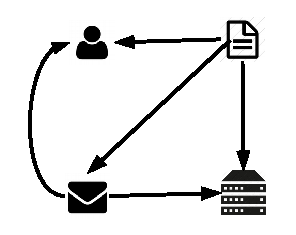
\includegraphics[scale=0.5]{gts/grammar/grammar-type-graph}}}
    \caption{Type Graph}
  \end{subfigure}
  \begin{subfigure}[t]{.5\textwidth}
    \centerline{\fbox{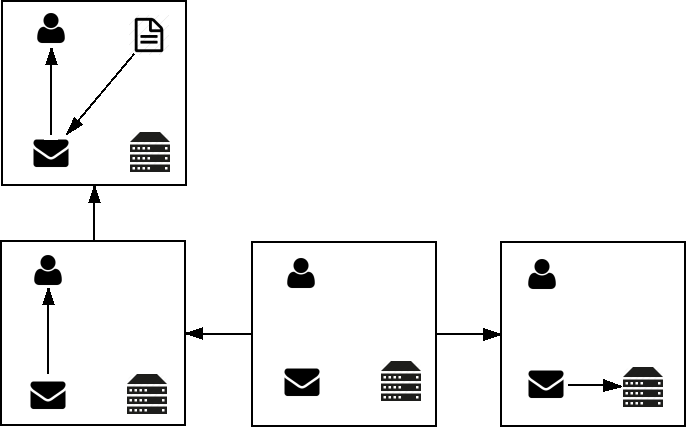
\includegraphics[scale=0.3]{gts/grammar/sendMessage}}}
    \caption{Send message}
  \end{subfigure}%
  \begin{subfigure}[t]{.5\textwidth}
    \centerline{\fbox{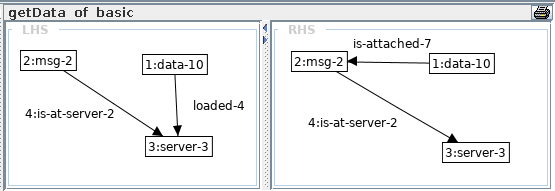
\includegraphics[scale=0.3]{gts/grammar/getData}}}
    \caption{Get data}
  \end{subfigure}
  \begin{subfigure}[t]{.5\textwidth}
    \centerline{\fbox{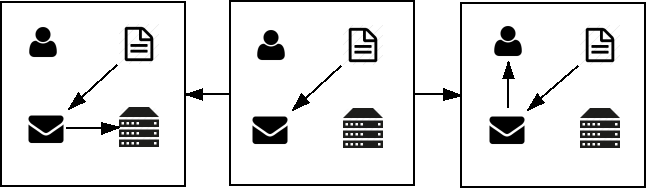
\includegraphics[scale=0.3]{gts/grammar/receiveMessage}}}
    \caption{Receive message}
  \end{subfigure}%
  \begin{subfigure}[t]{.5\textwidth}
    \centerline{\fbox{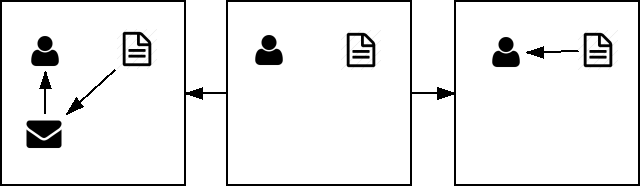
\includegraphics[scale=0.3]{gts/grammar/deleteMessage}}}
    \caption{Delete message}
  \end{subfigure}
  \caption{Mail application graph transformation system}\label{fig:gts:mail}
\end{figure}

\iffalse
\begin{figure}
\centering
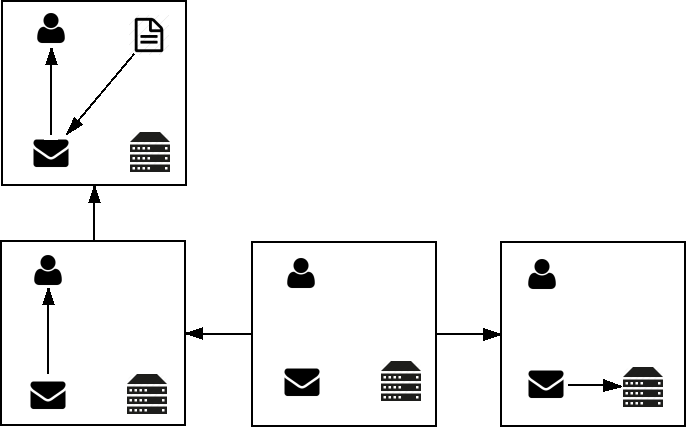
\includegraphics[width=6.5cm]{gts/grammar/sendMessage}
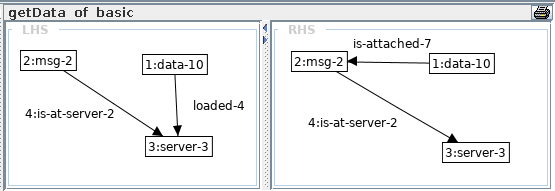
\includegraphics[width=5cm]{gts/grammar/getData}
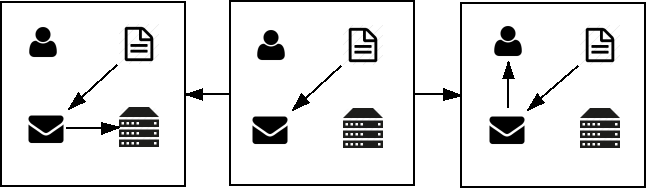
\includegraphics[width=5cm]{gts/grammar/receiveMessage}
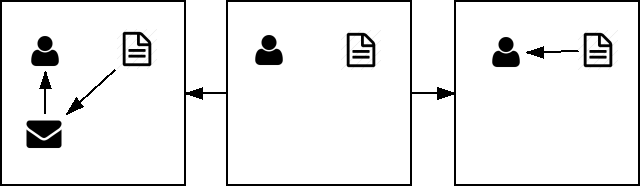
\includegraphics[width=5cm]{gts/grammar/deleteMessage}
\caption{\label{fig:gts:mail} Graph rules for Server}
\end{figure}
\fi
\end{example}

\section{Parallel and Sequential Independence}

One of the characteristics that make Graph Transformation Systems and Graph Grammars suitable formalisms to model and reason about parallel and/or concurrent systems is the possibility to check whether the transformations given by two graph rules over the same instance graph can be applied (1) at the same time or (2) in any interchangeable order. In the first case we say that the transformations are parallel independent; in the later we say that they are sequential independent.

In this section, we show both what it means for two graph transformations to be independent and how to check it. Notice that when we are reasoning about graph transformations (rules application) the (in)dependence is concrete, while for the case of graph rules the (in)dependence is potential, as it depends on the particular way the rules are applied.

\begin{definition}[Causal Dependency]\label{def:classic-dependency} Given two graph rules $p_1,p_2$ with NACs, they are \emph{causally dependent} for a given graph $E$, in which they overlap via morphisms \morph{m'_1}{R_1}{E} and \morph{m_2}{L_2}{E}, iff at least one of the following situations occurs in the transformations diagram below:

  \begin{enumerate}
    \item $\nexists h_{12} : R_1 -> D_2$ such that $d_2 \circ h_{12} = m_1'$
    \item $\exists! h_{12} : R_1 -> D_2$ such that $d_2 \circ h_{12} = m_1'$ but $e_2 \circ h_{12} \not\models NAC_{p_1^{-1}}$
    \item $\nexists h_{21} : L_2 -> D_1$ such that $e_1 \circ h_{21} = m_2$
    \item $\exists! h_{21} : L_2 -> D_1$ such that $e_1 \circ h_{21} = m_2$ but $d_1 \circ h_{21} \not\models NAC_{p_2}$
  \end{enumerate}

\diagram{
    N_1 & & & & N_2 & & \\
      L_1\ar[d]\ar[u]^{n_1} & K_1\ar[d]\ar[l]\ar[r] & R_1\ar[dr]_{m'_{1}}\ar@{.>}@/^1.1pc/[drrr]|<<{|}^<<<{h_{12}} & & L_2\ar[dl]^{m_2}\ar[u]^{n_2}\ar@{.>}@/_1.1pc/[dlll]|<<{|}_<<<{h_{21}} & K_2\ar[d]\ar[l]\ar[r] & R_2\ar[d]\\
        H_1 & D_1\ar[l]^{d_1}\ar[rr]_{e_1} & & \textit{E} & & D_2\ar[ll]^{d_2}\ar[r]_{e_2} & H_2\\
          & & & & & &
          }
\end{definition}

Intuitively, each case of dependency can be regarded as follows:

\begin{enumerate}
  \item a \emph{deliver-delete} dependency: $p_2$ deletes (from graph $E$) at least one element that was created or preserved by $p_1$.
  \item a \emph{forbid-produce} dependency: $p_2$ creates on $H_2$ at least one element that would trigger the NAC $N_1^{-1}$.
  \item a \emph{produce-use} dependency: $p_1$ creates (on graph $E$) at least one element needed for $p_2$ to be applied which did not exist on $H_1$.
  \item a \emph{delete-forbid} dependency: $p_1$ deletes (from graph $H_1$) at least one element that would trigger the NAC $N_2$, thus allowing the application of $p_2$ on $E$.
\end{enumerate}

\begin{example}[Dependency situation in the mail server grammar]
  Figure~\ref{fig:gts:dependency} shows a dependency situation between the rules \emph{getData} and \emph{receiveMessage}. In this case, the dependency is of a \emph{produce-use} kind: the edge between the \emph{piece of data} and the \emph{message} at the instance graph was created by \emph{getData} and the same edge is necessary for \emph{receiveMessage} to be applied.

\begin{figure}[!ht]
  \centering
  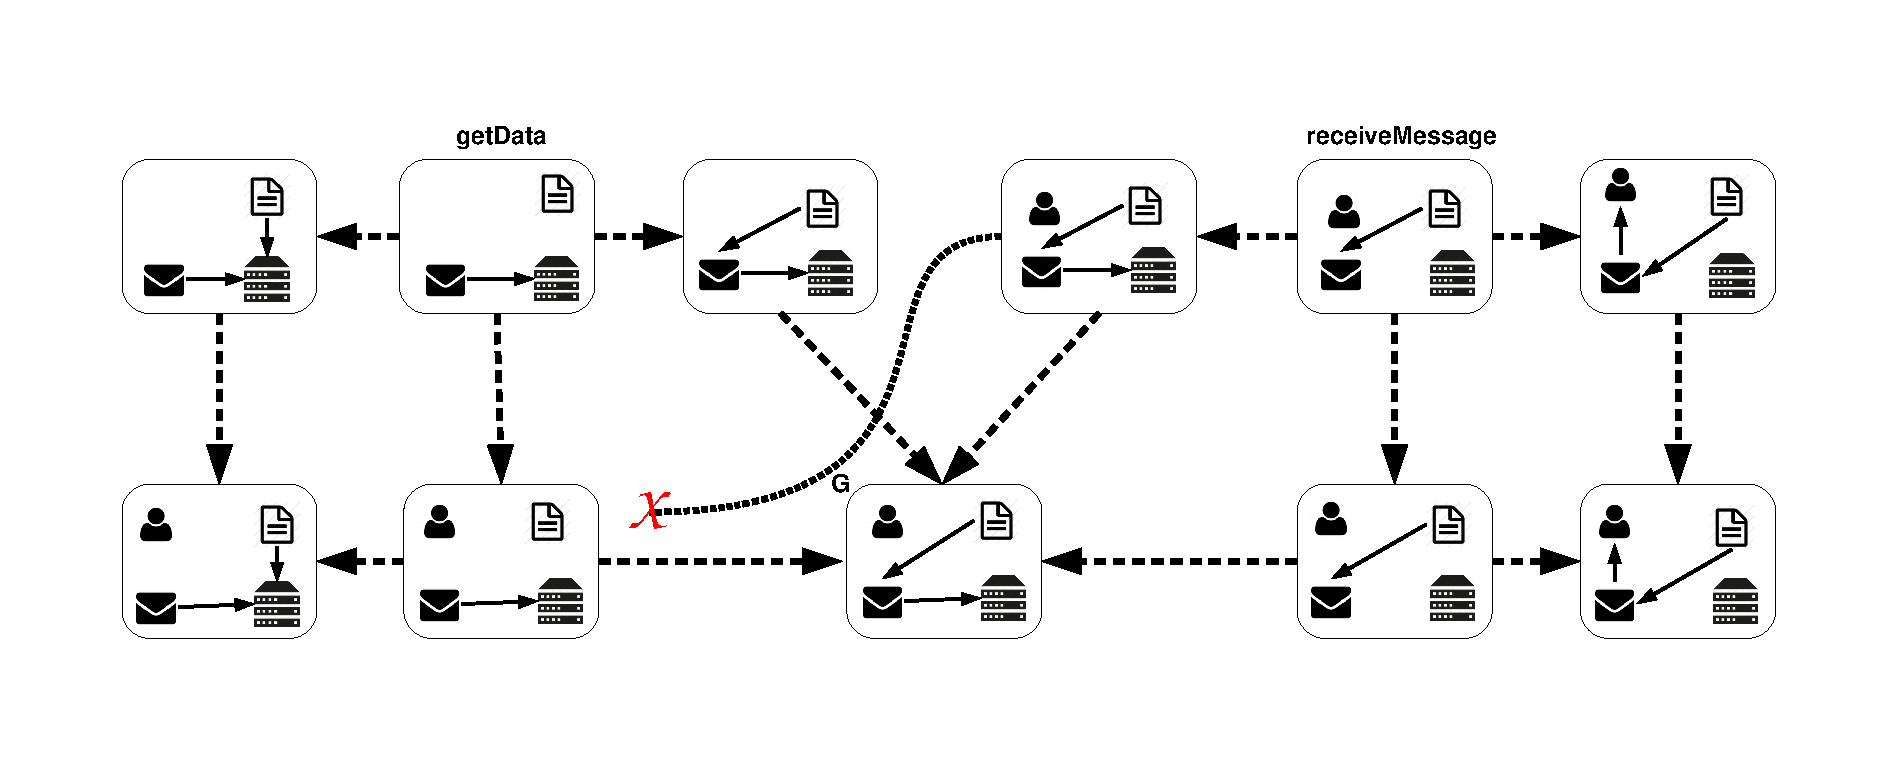
\includegraphics[scale=0.5]{images/gts/dependency}
  \caption{A dependency in the server grammar}\label{fig:gts:dependency}
\end{figure}

  In the diagram, it is not possible to find a morphism from the left-hand-side of \emph{receiveMessage} to the gluing graph of \emph{getData} such that the transformation is still valid. Thus, for the overlapping in this particular graph, \emph{receiveMessage} is causally dependent on \emph{getData}.
\end{example}

\begin{definition}[Conflict]\label{def:classic-conflict} Given two graph rules $p_1, p_2$ with NACs, they are in conflict for a given graph $E$, in which they overlap via morphisms \morph{m_1}{L_1}{E} and \morph{m_2}{L_2}{E}, iff at least one of the following situations occur:

\begin{enumerate}
    \item $\nexists h_{12} : L_1 -> D_2$ such that $d_2 \circ h_{12} = m_1$
    \item $\exists! h_{12} : R_1 -> D_2$ such that $d_2 \circ h_{12} = m_1$ but $e_2 \circ h_{12} \not\models NAC_{p_1}$
    \item $\nexists h_{21} : L_2 -> D_1$ such that $d_1 \circ h_{21} = m_2$
    \item $\exists! h_{21} : L_2 -> D_1$ such that $d_1 \circ h_{21} = m_2$ but $e_1 \circ h_{21} \not\models NAC_{p_2}$
  \end{enumerate}

\diagram{
     & & N_1 & & N_2 & & \\
      R_1\ar[d] & K_1\ar[d]\ar[l]\ar[r] & L_1\ar[u]^{n_1}\ar[dr]^{m_1}\ar@{.>}@/^1.1pc/[drrr]|<<{|}^<<<{h_{12}} & & L_2\ar[dl]_{m_2}\ar[u]^{n_2}\ar@{.>}@/_1.1pc/[dlll]|<<{|}_<<<{h_{21}} & K_2\ar[d]\ar[l]\ar[r] & R_2\ar[d]\\
        H_1 & D_1\ar[l]^{e_1}\ar[rr]_{d_1} & & \textit{E} & & D_2\ar[ll]^{d_2}\ar[r]_{e_2} & H_2\\
          & & & & & &
          }
\end{definition}

Intuitively, each conflict case can be regarded as:

\begin{enumerate}
  \item a \emph{delete-use} conflict: $p_2$ deletes (from graph $E$) at least one element needed for $p_1$ to be applied.
  \item a \emph{produce-forbid} conflict: $p_2$ produces (on graph $H_2$) at least one element that triggers the NAC $N_1$.
  \item a \emph{delete-use} conflict: $p_1$ deletes at least one element needed for $p_2$ to be applied
  \item a \emph{produce-forbid} conflict: $p_1$ creates at least one element that triggers the NAC $N_2$.
\end{enumerate}

\begin{example}[Conflict situation in the mail server grammar]
  Figure~\ref{fig:gts:dependency} shows a conflict situation involving the rules \emph{getData} and \emph{receiveMessage}. This is a \emph{delete-use} conflict: \emph{receiveMessage} deletes from the overlapping graph an edge between the \emph{message} and the \emph{server} which is necessary for \emph{getData} to be applied. Both rules are applied over the same graph and, individually, both transformations are valid. However, once \emph{receiveMessage} is applied, it is no longer possible to
  apply \emph{getData}. This is represented in the diagram by the fact that it is not possible to find a morphism from the left-hand-side of \emph{getData} to the gluing graph of \emph{receiveMessage} such that the transformation from there is still valid.

\begin{figure}[!ht]
  \centering
  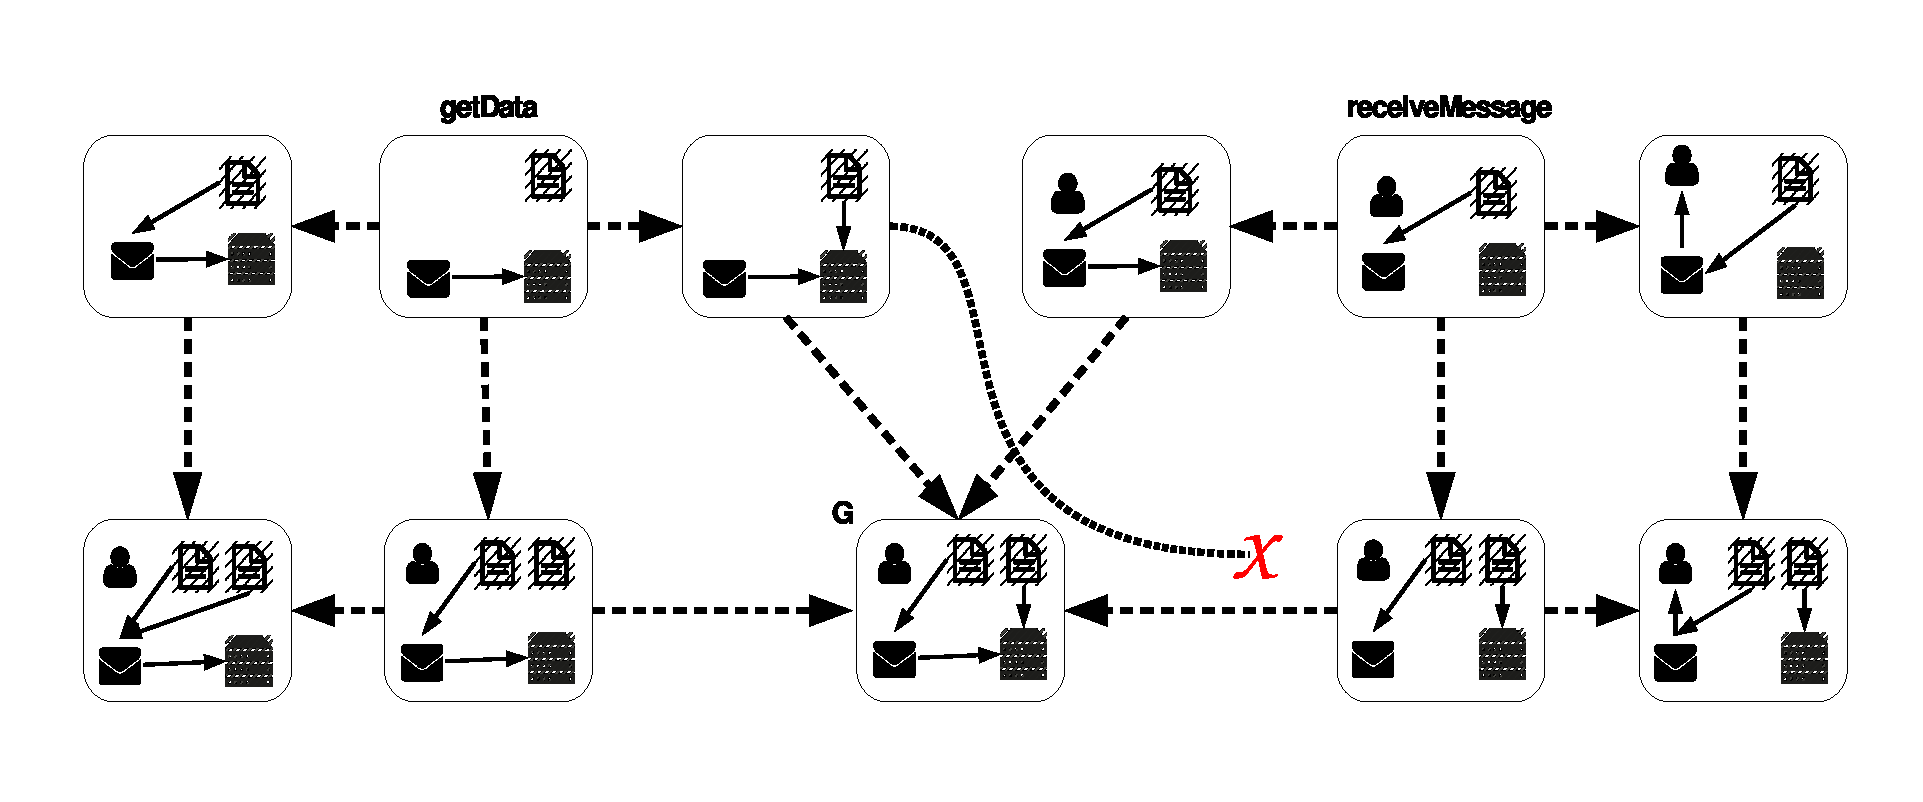
\includegraphics[scale=0.5]{images/gts/conflict}
  \caption{A conflict in the server grammar}\label{fig:gts:conflict}
\end{figure}

\end{example}
